\documentclass[usenames,dvipsnames]{article}

\usepackage{pgf}
\usepackage{tikz}
\usetikzlibrary{arrows,automata}
\usepackage[latin1]{inputenc}
\usepackage{verbatim}
\usepackage{xcolor}
\newcommand{\lightgrey}{black!10}
\newcommand{\darkgrey}{black!40}
\begin{document}
  \pagestyle{empty}
  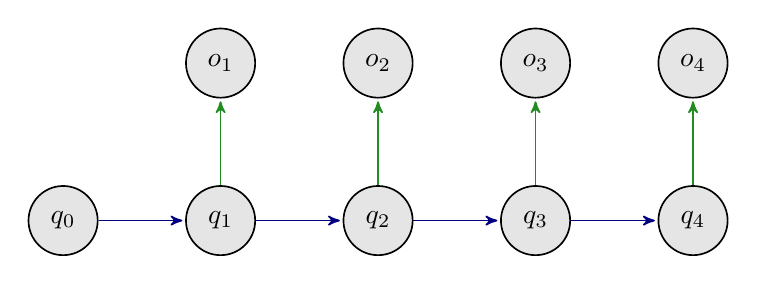
\begin{tikzpicture}[->,>=stealth',shorten >=1pt,auto,node distance=4cm,semithick]
    \tikzstyle{every state}=[fill=\lightgrey,draw=black,text=black]
    \tikzset{every loop/.style={min distance=10mm,looseness=10}}
    \node[state] (q0) at (0, 0) {$q_0$};
    \node[state] (q1) at (2, 0) {$q_1$};
    \node[state] (o1) at (2, 2) {$o_1$};
    \node[state] (q2) at (4, 0) {$q_2$};
    \node[state] (o2) at (4, 2) {$o_2$};
    \node[state] (q3) at (6, 0) {$q_3$};
    \node[state] (o3) at (6, 2) {$o_3$};
    \node[state] (q4) at (8, 0) {$q_4$};
    \node[state] (o4) at (8, 2) {$o_4$};
    \path (q0) edge [draw=NavyBlue] node {} (q1);
    \path (q1) edge [draw=ForestGreen] node {} (o1);
    \path (q1) edge [draw=NavyBlue] node {} (q2);
    \path (q2) edge [draw=ForestGreen] node {} (o2);
    \path (q2) edge [draw=NavyBlue] node {} (q3);
    \path (q3) edge [draw=ForestGreen] node {} (o3);
    \path (q3) edge [draw=NavyBlue] node {} (q4);
    \path (q4) edge [draw=ForestGreen] node {} (o4);
  \end{tikzpicture}
\end{document}
